\documentclass{article} % What kind of document this is
\usepackage{tikz} % Import the tikz package
\usetikzlibrary{automata} % Import library for drawing automata
\usetikzlibrary{positioning} % ...positioning nodes
\usetikzlibrary{arrows} % ...customizing arrows
\tikzset{node distance=2.5cm, % Minimum distance between two nodes. Change if necessary.
every state/.style={ % Sets the properties for each state
semithick,
fill=gray!10},
initial text={}, % No label on start arrow
double distance=2pt, % Adjust appearance of accept states
every edge/.style={ % Sets the properties for each transition
draw,
->, % Makes edges directed with bold arrowheads
auto,
semithick}}
\let\epsilon\varepsilon

\begin{document}


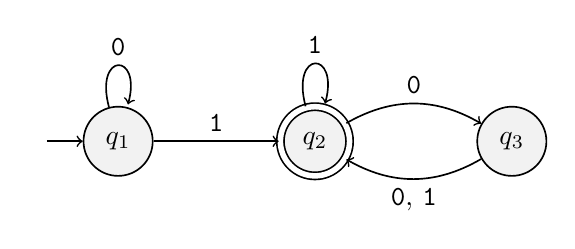
\begin{tikzpicture}
\node[state, initial] (q1) {$q_1$};
\node[state, accepting, right of=q1] (q2) {$q_2$};
\node[state, right of=q2] (q3) {$q_3$};
\draw (q1) edge[loop above] node {\tt 0} (q1);
\draw (q1) edge node {\tt 1} (q2);
\draw (q2) edge[loop above] node {\tt 1} (q2);
\draw (q2) edge[bend left] node {\tt 0} (q3);
\draw (q3) edge[bend left] node {{\tt 0}, {\tt 1}} (q2);
\end{tikzpicture}



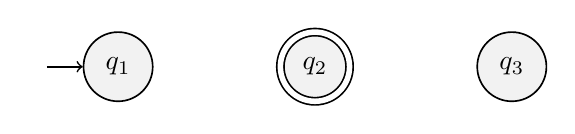
\begin{tikzpicture}
\node[state, initial] (q1) {$q_1$};
\node[state, accepting, right of=q1] (q2) {$q_2$};
\node[state, right of=q2] (q3) {$q_3$};
\end{tikzpicture}



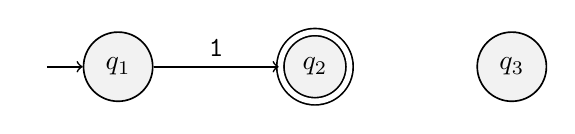
\begin{tikzpicture}
\node[state, initial] (q1) {$q_1$};
\node[state, accepting, right of=q1] (q2) {$q_2$};
\node[state, right of=q2] (q3) {$q_3$};
\draw (q1) edge node {\tt 1} (q2);
\end{tikzpicture}




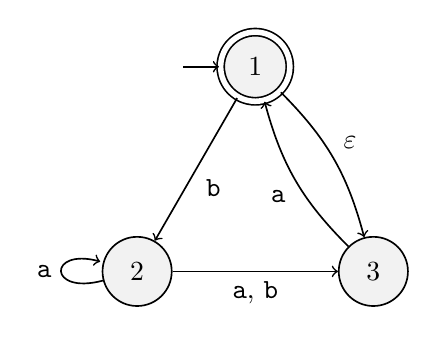
\begin{tikzpicture}
\node[state, initial, accepting] (1) at (1.5,2.6) {$1$};
\node[state] (2) at (0,0) {$2$};
\node[state] (3) at (3,0) {$3$};
\draw (1) edge node{\tt b} (2)
edge[bend left=15] node {$\epsilon$} (3)
(2) edge[loop left] node{\tt a} (2)
edge[below] node{{\tt a}, {\tt b}} (3)
(3) edge[bend left=15] node{\tt a} (1);
\end{tikzpicture}






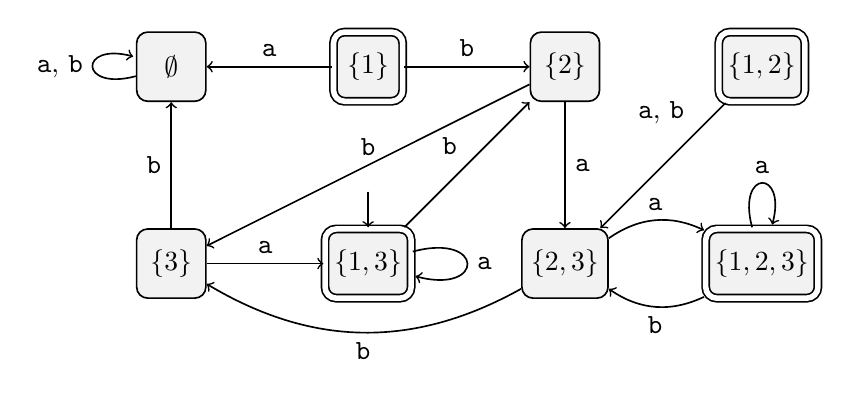
\begin{tikzpicture}
\tikzset{every state/.append style={rectangle, rounded corners}}
\node[state] (emp) {$\emptyset$};
\node[state, accepting, right of=emp] (1) {$\{1\}$};
\node[state, right of=1] (2) {$\{2\}$};
\node[state, accepting, right of=2] (12) {$\{1, 2\}$};
\node[state, below of=emp] (3) {$\{3\}$};
\node[state, initial, initial where=above, accepting, right of=3] (13) {$\{1, 3\}$};
\node[state, right of=13] (23) {$\{2, 3\}$};
\node[state, accepting, right of=23] (123) {$\{1, 2, 3\}$};
\draw (emp) edge[loop left] node {{\tt a}, {\tt b}} (emp)
(1) edge[above] node {\tt a} (emp)
(1) edge node {\tt b} (2)
(2) edge node {\tt a} (23)
(2) edge[above] node {\tt b} (3)
(12) edge[auto=right,near start] node {{\tt a}, {\tt b}} (23)
(3) edge node {\tt b} (emp)
(3) edge node {\tt a} (13)
(13) edge[loop right] node {\tt a} (13)
(13) edge node {\tt b} (2)
(23) edge[bend left,above] node {\tt a} (123)
(23) edge[bend left] node {\tt b} (3)
(123) edge[loop above] node {\tt a} (123)
(123) edge[bend left,below] node {\tt b} (23);
\end{tikzpicture}



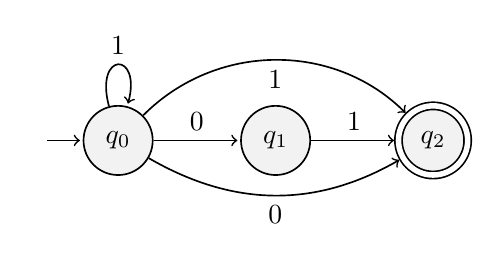
\begin{tikzpicture}[shorten >=1pt,node distance=2cm,on grid]
  \node[state,initial]   (q_0)                {$q_0$};
  \node[state]           (q_1) [right=of q_0] {$q_1$};
  \node[state,accepting] (q_2) [right=of q_1] {$q_2$};
  \path[->] (q_0) edge                node [above] {0} (q_1)
                  edge [loop above]   node         {1} ()
                  edge [bend left=45] node [below] {1} (q_2)
                  edge [bend right]   node [below] {0} (q_2)
            (q_1) edge                node [above] {1} (q_2);
\end{tikzpicture}




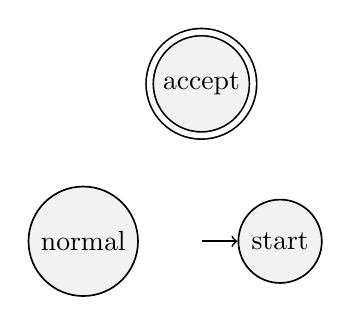
\begin{tikzpicture}
\node[state] (q1) {normal};
\node[state, initial, right of=q1] (q2) {start};
\node[state, accepting] at (1.5, 2) (q3) {accept};
\end{tikzpicture}






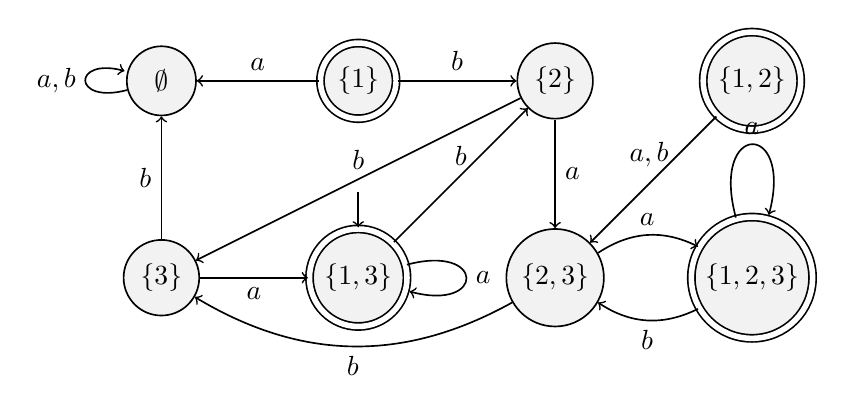
\begin{tikzpicture}
\node[state] (phi) {$\emptyset$};
\node[state, accepting, right of=phi] (1) {$\{1\}$};
\node[state, right of=1] (2) {$\{2\}$};
\node[state, accepting, right of=2] (12) {$\{1, 2\}$};
\node[state, below of=phi] (3) {$\{3\}$};
\node[state, initial, initial where=above, accepting, right of=3] (13) {$\{1, 3\}$};
\node[state, right of=13] (23) {$\{2, 3\}$};
\node[state, accepting, right of=23] (123) {$\{1, 2, 3\}$};
5
\draw (phi) edge[loop left] node{$a, b$} (phi)
(1) edge[above] node{$a$} (phi)
(1) edge[above] node{$b$} (2)
(2) edge[right] node{$a$} (23)
(2) edge[above] node{$b$} (3)
(12) edge[above, pos=.3, left=2pt] node{$a, b$} (23)
(3) edge[left] node{$b$} (phi)
(3) edge[below] node{$a$} (13)
(13) edge[loop right] node{$a$} (13)
(13) edge[above] node{$b$} (2)
(23) edge[bend left, above] node{$a$} (123)
(23) edge[bend left, below] node{$b$} (3)
(123) edge[loop above] node{$a$} (123)
(123) edge[bend left, below] node{$b$} (23);
\end{tikzpicture}











\end{document}